\subsubsection{Controllers}
Vengono di seguito riportate alcune sequenze di operazioni svolte dai controller che si è ritenuto utile descrivere più in dettaglio.

\paragraph{5.1.1.1 Ricerca}\mbox{}\\

\noindent Il diagramma sottostante rappresenta le operazioni che vengono eseguite quando un utente effettua una ricerca. La sequenza di operazioni che portano a mostrare i risultati di una ricerca ha inizio dopo che l'utente ha inserito una chiave di ricerca nell'apposita form nella home page, ha settato il filtro per la ricerca ed ha premuto il tasto \textbf{Search}. Vengono quindi passati tutti i parametri della ricerca a \textit{HomePageCtrl} che, a seconda che il filtro sia settato su Users o Project, invoca rispettivamente searchByUsers() oppure searchByProject(). Indipendentemente da quale dei due metodi viene invocato, \textbf{ProjectService} inanzitutto chiama resetSearchResults() per eliminare i risultati di eventuali ricerche precedenti, poi elabora i dati e scrive i nuovi risultati della ricerca in searchResults(), che li ritorna a \textbf{HomePageCtrl}. Qui la view riguardante la ricerca viene aggiornata con un refresh() che mostra i nuovi risultati.

\begin{figure}[H] 
	\centering 
	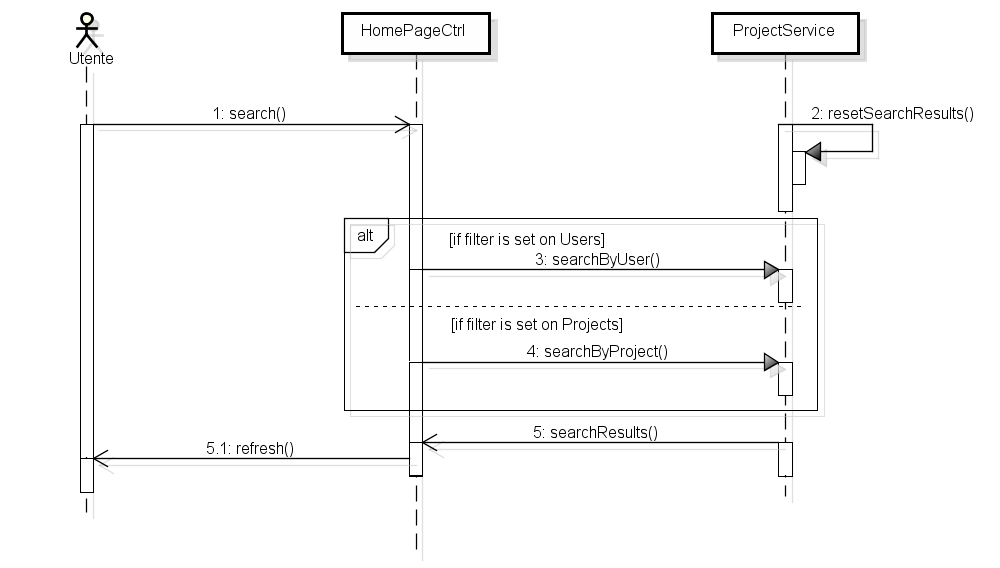
\includegraphics[scale=0.60] {img/ricerca.png}
	\caption{Diagrammi di sequenza front-end - Ricerca} 
\end{figure}


\newpage
\paragraph{5.1.1.2 Inserimento dati real time}\mbox{}\\

\noindent Il diagramma sottostante rappresenta le operazioni che vengono eseguite quando un utente inserisce dei dati real time all'interno di una slide. La sequenza di operazioni che portano a mostrare i risultati di una ricerca ha inizio dopo che l'utente ha premuto il bottone di inserimento dati real time nell'editor delle slide, ha riempito i campi richiesti dal form che appare ed ha premuto il bottone \textbf{Insert}. I dati inseriti vengono raccolti da addRealTimeData() che li invia a \textbf{ComponentCtrl}. Ogni dato raccolto viene controllato dal proprio metodo (target da targetUrl(), selector da selector() e così via) e settato dal rispettivo metodo (target da setTargetUrl(), selector da setSelector() e così via). Una volta raccolti i dati vengono inviati a RealTimeDataService() che li processa, e se risultano esatti risponde con un \textit{True} aggiungendo i dati real time alla slide, in caso contrario risponde con un \textit{false} e viene segnalato con un  messaggio di errore.

\begin{figure}[H] 
	\centering 
	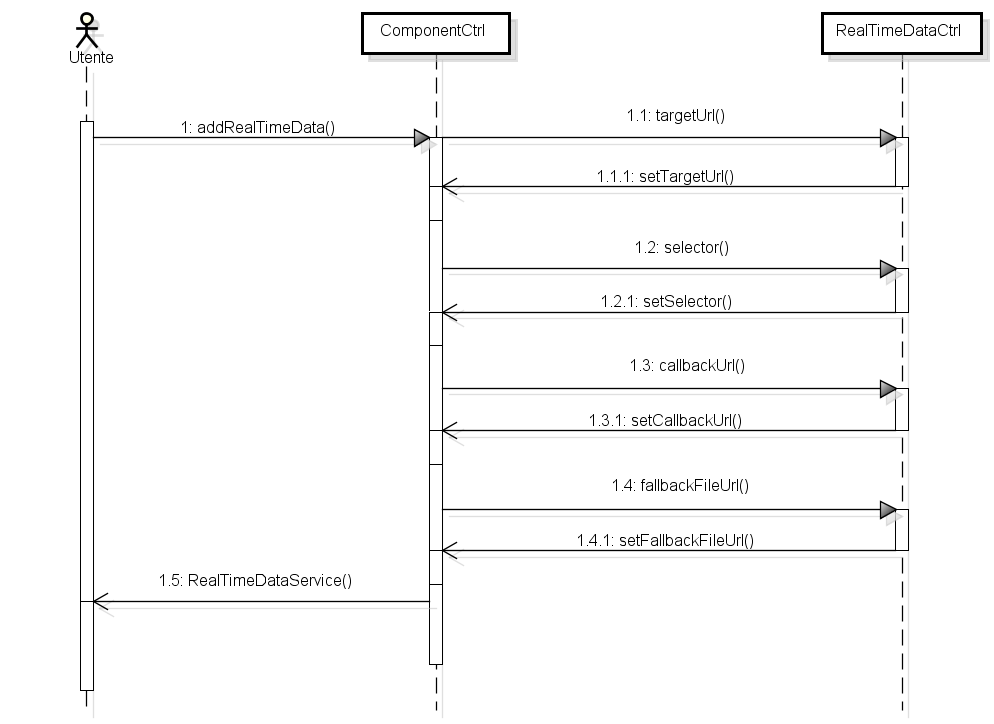
\includegraphics[scale=0.60] {img/realtime.png}
	\caption{Diagrammi di sequenza front-end - Inserimento dati real time} 
\end{figure}